\documentclass[14pt, a4paper]{extarticle}
\usepackage[T2A]{fontenc}
\usepackage[utf8]{inputenc}
\usepackage[english,russian]{babel}
\usepackage[left = 3cm, right = 1cm, top = 2cm, bottom = 2cm]{geometry}
\setlength\parindent{12.5mm} 
\linespread{1.3}
\usepackage{enumitem}
\usepackage{amsmath}
\usepackage{amssymb}
\usepackage{wrapfig}
\usepackage{indentfirst}
\usepackage{hyperref}
\hypersetup{
	colorlinks=true,
	citecolor=blue,
	urlcolor=blue, 
	linkcolor=blue,
	pdfencoding=auto
}
\usepackage{xcolor}
\usepackage{listings}
\usepackage{graphicx}
\usepackage{float}
\usepackage{longtable}
\usepackage[htt]{hyphenat}

\definecolor{codegreen}{rgb}{0,0.6,0}
\definecolor{codegray}{rgb}{0.5,0.5,0.5}
\definecolor{codepurple}{rgb}{0.58,0,0.82}
\definecolor{backcolour}{rgb}{0.97,0.97,0.97}

\lstset{ 
	language=C++,
	backgroundcolor=\color{backcolour},
	commentstyle=\color{codegreen}\itshape,
	keywordstyle=\color{blue}\bfseries,
	numberstyle=\tiny\color{codegray},
	stringstyle=\color{codepurple},
	basicstyle=\ttfamily\footnotesize,
	breakatwhitespace=false,         
	breaklines=true,
	captionpos=t,
	keepspaces=false,                   % КРИТИЧНО: отключает вставку \lst@FillFixed@
	columns=fullflexible,               % КРИТИЧНО: отключает посимвольную сетку знакомест
	extendedchars=false,                % КРИТИЧНО: именно false для работы с utf8 в pdflatex
	numbers=left,
	numbersep=10pt,
	showspaces=false,                
	showstringspaces=false,
	showtabs=false,                  
	tabsize=4,
	frame=single,
	rulecolor=\color{black!30}
}
\newcommand{\tab}{\hspace{12.5mm}}

\begin{document}
	\thispagestyle{empty}
	\begin{center}
		\hspace{0.2cm}МИНИСТЕРСТВО НАУКИ И ВЫСШЕГО ОБРАЗОВАНИЯ РОССИЙСКОЙ ФЕДЕРАЦИИ\\
		Федеральное государственное автономное образовательное\\
		учреждение высшего образования\\
		{\bf <<Санкт-Петербургский политехнический\\
			университет Петра Великого>>}\\
		Институт компьютерных наук и кибербезопасности\\
		Высшая школа технологий искусственного интеллекта\\
		02.03.01\_03 Технологии машинного обучения и искусственного интеллекта\\
		\vspace{2.5cm}
		\Large\bf{
			Отчёт по лабораторной работе № 1 \\
			по дисциплине <<Дискретная математика>>\\[0.8cm]
			<<Операции над мультимножествами и генерация бинарного кода Грея>>\\[1cm]
		}
	\end{center}
	\vspace{1.5cm}
	\begin{flushleft}
		{\bf Выполнил:}\\
		Cтудент группы 5130201/50302 \hfill
		\line(1,0){4cm} \quad Калинский В.И.\\
		{\bf Принял:}\\
		Преподаватель \hfill
		\line(1,0){4 cm} \quad Востров А.В.\\[0.5cm]
		{ \hfill<<\rule{1cm}{0.5pt}>>\rule{2cm}{0.5pt}\hspace{3pt}2026 г.}
	\end{flushleft}
	\vspace{1cm}
	\begin{center}
		Санкт-Петербург, 2026
	\end{center}
	\newpage
	
	\tableofcontents
	
	\newpage
	\thispagestyle{empty}
	\phantomsection
	\addcontentsline{toc}{section}{Введение}
	{\LARGE\bf Введение}\\
	
	В современной дискретной математике и информатике классическая теория множеств часто оказывается недостаточной для описания реальных информационных структур. Во многих задачах возникает необходимость оперировать наборами элементов, в которых один и тот же объект может присутствовать многократно. Такие математические объекты называются \textit{мультимножествами}.
	
	Для практического применения мультимножеств в вычислительных системах требуется определить конечное базовое множество(носитель) и универсальное мультимножество(универсум), относительно которого корректно определяются операции на мультимножествах. В качестве эффективного базиса для формирования универсума в данной работе выступает двоичный код Грея.
	
	{\bf Цель работы:} изучение алгебраических и теоретико-множественных свойств мультимножеств, освоение алгоритмов генерации перестановок и кодов Грея, а также программная реализация консольного приложения для моделирования операций над мультимножествами.
	
	{\bf Постановка задачи:}
	\begin{enumerate}[label=\arabic*.]
				\item Разработать алгоритм и программный модуль генерации $n$-разрядного бинарного кода Грея, где разрядность $n \in [0, 27]$ задается пользователем. Верхняя граница разрядности выбрана исходя из критерия времени генерации до 5 секунд (при $n = 28$ среднее время составляет 7.3 с, при $n = 27$ -- 3.6 с). Предусмотреть обработку краевого случая пустого универсума при $n = 0$.
		\item Сформировать упорядоченный универсум $U$, кратности элементов которого генерируются случайным образом в диапазоне от 1 до 10 (при $n = 0$ универсум пуст).
		\item Реализовать создание двух мультимножеств $A$ и $B$ над построенным носителем с мощностями, задаваемыми пользователем в диапазоне от 0 до доступной суммарной емкости универсума (не более 100).
		\item Предусмотреть два альтернативных режима наполнения мультимножеств:
		\begin{itemize}
			\item ручной ввод пользователем (выбор номера элемента носителя и задание его кратности с контролем непревышения как целевой мощности, так и доступной емкости элемента в универсуме);
			\item автоматическая генерация кратностей элементов на основе датчика псевдослучайных чисел с контролем лимитов универсума.
		\end{itemize}
		\item Реализовать вычисление следующих операций над мультимножествами:
		\begin{itemize}
			\item объединение ($A \cup B$);
			\item пересечение ($A \cap B$);
			\item разность в обоих направлениях ($A \setminus B$ и $B \setminus A$);
			\item симметрическая разность ($A \triangle B$);
			\item дополнение до универсума ($\overline{A} = U \setminus A$ и $\overline{B} = U \setminus B$);
			\item арифметическая сумма ($A + B$);
			\item арифметическая разность ($A - B$ и $B - A$);
			\item арифметическое произведение ($A \cdot B$);
			\item арифметическое деление ($A : B$ и $B : A$).
		\end{itemize}
		\item Предусмотреть ограничение вывода мультимножеств в консоль, строгую фильтрацию некорректного пользовательского ввода и интерактивное меню управления.
	\end{enumerate}
	
	\newpage
	\newpage
	\section{Математическое описание}
	
	\subsection{Понятие множества, мультимножества и универсума}
	
	Классическим \textit{множеством} называется совокупность определенных, различимых объектов (элементов), мыслимая как единое целое, причем каждый элемент либо принадлежит множеству, либо не принадлежит ему.
	
	\textit{Мультимножеством} над базовым множеством $X = \{x_1, x_2, \dots, x_N\}$ называется пара $\hat{A} = (X, k_A)$, где $k_A: X \to \mathbb{N} \cup \{0\} $ -- характеристическая функция кратности, сопоставляющая каждому элементу $x_i \in X$ целое неотрицательное число $\alpha_i \ge 0$, называемое \textit{кратностью} (степенью вхождения) элемента в мультимножество. 
	
	Символически мультимножество записывается в виде:
	\begin{equation}
		\hat{A} = \{x_1^{\alpha_1}, x_2^{\alpha_2}, \dots, x_N^{\alpha_N}\}, \quad \alpha_i \in [0, k],
	\end{equation}
	где $x_i^{\alpha_i}$ обозначает вхождение элемента $x_i$ ровно $\alpha_i$ раз. Если $\alpha_i = 0$, элемент фактически отсутствует в мультимножестве. Пустое мультимножество обозначается вектором нулевых кратностей: $\varnothing = (0, 0, \dots, 0)$.
	
	\textit{Мощностью мультимножества} $|\hat{A}|$ называется сумма кратностей всех его элементов:
	\begin{equation}
		|\hat{A}| = \sum_{i=1}^{N} k_A(x_i) = \sum_{i=1}^{N} \alpha_i.
	\end{equation}
	
	\textit{Универсумом мультимножеств} $U$ называется фиксированное мультимножество над тем же носителем $X$:
	\begin{equation}
		U = \{x_1^{m_1}, x_2^{m_2}, \dots, x_N^{m_N}\}, \quad m_i \ge 0,
	\end{equation}
	ограничивающее сверху максимальную кратность элементов любого рассматриваемого мультимножества: $\forall i \; (\alpha_i \le m_i)$.
	
	В рамках разработанной программы универсум $U$ формируется следующим образом: кратности его элементов $m_i$ задаются псевдослучайными числами в диапазоне от 1 до 10:
	\begin{equation}
		U = \{x_1^{m_1}, x_2^{m_2}, \dots, x_N^{m_N}\}, \quad m_i \in [1, 10].
	\end{equation}
	В краевом случае нулевой разрядности кода Грея ($n = 0$) носитель элементов отсутствует, универсум является пустым ($U = \varnothing$, $|U| = 0$), а мультимножества $A$ и $B$ автоматически инициализируются как пустые.
	
	\subsection{Теоретико-множественные и арифметические операции}
	
	Пусть $A = \{x_i^{\alpha_1}\}$ и $B = \{x_i^{\alpha_2}\}$ -- два мультимножества над носителем $X$, а $U = \{x_i^{m_i}\}$ -- универсум с кратностями $m_i \in [1, 10]$. Правила вычисления кратностей результирующих мультимножеств определяются следующим образом:
	
	\begin{enumerate}
		\item {\bf Пересечение ($A \cap B$):}
		Кратность каждого элемента равна минимальной из кратностей в операндах:
		\begin{equation}
			k_{A \cap B}(x_i) = \min(\alpha_{1,i}, \alpha_{2,i}).
		\end{equation}
		
		\item {\bf Объединение ($A \cup B$):}
		Кратность каждого элемента равна максимальной из кратностей в операндах:
		\begin{equation}
			k_{A \cup B}(x_i) = \max(\alpha_{1,i}, \alpha_{2,i}).
		\end{equation}
		
		\item {\bf Дополнение ($\overline{A}$ и $\overline{B}$):}
		Дополнение мультимножества вычисляется относительно универсума $U$:
		\begin{equation}
			k_{\overline{A}}(x_i) = m_i - \alpha_{1,i}, \quad k_{\overline{B}}(x_i) = m_i - \alpha_{2,i}.
		\end{equation}
		
		\item {\bf Разность ($A \setminus B$ и $B \setminus A$):}
		В теоретическом конспекте разность определяется через пересечение с дополнением: $A \setminus B = A \cap \overline{B}$. Подставляя формулу дополнения, получаем:
		\begin{equation}
			k_{A \setminus B}(x_i) = \min(\alpha_{1,i}, m_i - \alpha_{2,i}).
		\end{equation}
		Аналогично, для обратной разности:
		\begin{equation}
			k_{B \setminus A}(x_i) = \min(\alpha_{2,i}, m_i - \alpha_{1,i}).
		\end{equation}
		
		\item {\bf Симметрическая разность ($A \triangle B$):}
		Определяется как разность между объединением и пересечением мультимножеств:
		\begin{equation}
			A \triangle B = (A \cup B) \setminus (A \cap B) = (A \cup B) \cap \overline{(A \cap B)}.
		\end{equation}
		Кратность элемента:
		\begin{equation}
			k_{A \triangle B}(x_i) = \min\Big(\max(\alpha_{1,i}, \alpha_{2,i}), \; m_i - \min(\alpha_{1,i}, \alpha_{2,i})\Big).
		\end{equation}
		
		\item {\bf Арифметическая сумма ($A + B$):}
		Кратность каждого элемента в сумме мультимножеств ограничивается сверху его максимальной кратностью в универсуме $U$:
		\begin{equation}
			k_{A + B}(x_i) = \min(\alpha_{1,i} + \alpha_{2,i}, \; m_i).
		\end{equation}
		
		\item {\bf Арифметическая разность ($A - B$ и $B - A$):}
		Кратность представляет собой усеченную разность (не может быть отрицательной):
		\begin{equation}
			k_{A - B}(x_i) = \max(0, \alpha_{1,i} - \alpha_{2,i}),
		\end{equation}
		\begin{equation}
			k_{B - A}(x_i) = \max(0, \alpha_{2,i} - \alpha_{1,i}).
		\end{equation}
		
		\item {\bf Арифметическое произведение ($A \cdot B$):}
		Поэлементное произведение кратностей с обязательным ограничением сверху кратностью универсума $U$:
		\begin{equation}
			k_{A \cdot B}(x_i) = \min(\alpha_{1,i} \cdot \alpha_{2,i}, m_i).
		\end{equation}
		
		\item {\bf Арифметическое деление ($A : B$ и $B : A$):}
		Целочисленное деление кратностей. В соответствии с договоренностью при делении на 0 результирующая кратность принимается равной 0:
		\begin{equation}
			k_{A / B}(x_i) = \begin{cases}
			 \alpha_{1,i} / \alpha_{2,i} , & \alpha_{2,i} \ne 0, \\
				0, & \alpha_{2,i} = 0.
			\end{cases}
		\end{equation}
		\begin{equation}
			k_{B / A}(x_i) = \begin{cases}
				 \alpha_{2,i} / \alpha_{1,i} , & \alpha_{1,i} \ne 0, \\
				0, & \alpha_{1,i} = 0.
			\end{cases}
		\end{equation}
	\end{enumerate}
	
	\subsection{Алгоритм генерации бинарного кода Грея}
	
	Бинарным кодом Грея порядка $n$ называется последовательность всех $2^n$ двоичных векторов длины $n$, упорядоченная таким образом, что любые два соседних кода, а также первый и последний, отличаются ровно на один разряд.
	
	Для генерации последовательности кодовых слов используется алгоритм, описанный в фундаментальном учебнике Ф.\,А.~Новикова <<Дискретная математика для программистов>>~\cite{novikov}. Согласно данному алгоритму, переход от кодового слова $B_{i-1}$ к следующему кодовому слову $B_i$ ($i = 1, 2, \dots, 2^n - 1$) осуществляется инверсией бита с индексом $p = Q(i) - 1$, где функция $Q(i)$ возвращает номер младшей единицы в двоичной записи шага $i$:
	\begin{equation}
		Q(i) = 1 + \max \{k \in \mathbb{N} \cup \{0\} \mid i \text{ делится на } 2^k\}.
	\end{equation}
	
	Алгоритмически вычисление $Q(i)$ представляет собой подсчет числа делений $i$ на 2 до получения нечетного остатка:
	\begin{equation}
		\begin{cases}
			q = 1, \quad j = i; \\
			\text{пока } (j \pmod 2 == 0): \quad j = j / 2, \quad q = q + 1; \\
			\text{возврат } q.
		\end{cases}
	\end{equation}
	
	Тогда закон формирования кодовой последовательности имеет вид:
	\begin{equation}
		B_0 = 0, \quad B_i = B_{i-1} \oplus (1 \ll (Q(i) - 1)), \quad i = 1, \dots, 2^n - 1,
	\end{equation}
	где $\oplus$ -- побитовая операция XOR, $\ll$ -- побитовый сдвиг влево. Вектор сгенерированных целых чисел служит базисом упорядоченного универсума.
	
	Разрядность генерируемого кода ограничена диапазоном $n \in [0, 27]$. Выбор верхней границы обусловлен временным критерием: время построения носителя не должно превышать 5 секунд. В ходе экспериментальных замеров при $n = 28$ среднее время работы генератора составило 7.3 секунды, тогда как при $n = 27$ оно составило 3.6 секунды, что удовлетворяет установленному критерию быстродействия. При $n = 0$ генерация не выполняется, и универсум остаётся пустым.
	
	\newpage
	\newpage
	\section{Особенности реализации}
	
	\subsection{Архитектура программного комплекса и структуры данных}
	
	Программный комплекс спроектирован на языке C++ (стандарт C++20) в соответствии с принципами модульности и разделения ответственности:
	\begin{itemize}
		\item \texttt{MultiSet.hpp} -- спецификация интерфейса класса мультимножества и внешних операторов;
		\item \texttt{MultiSet.cpp} -- реализация операций над мультимножествами с применением алгоритмов стандартной библиотеки шаблонов STL\\ (\texttt{std::transform});
		\item \texttt{main.cpp} -- модуль консольного взаимодействия, генерации кода Грея, ввода данных и управления логикой;
		\item \texttt{CMakeLists.txt} -- сценарий автоматизированной сборки проекта со статической линковкой библиотеки \texttt{mylib} и интеграцией динамического санитайзера памяти AddressSanitizer (\texttt{-fsanitize=address -fno-omit-frame-pointer -O1}).
	\end{itemize}
	
	Основной структурой данных для представления мультимножества выступает класс \texttt{MultiSet}, являющийся адаптером \textit{std::vector<int>}. Внутреннее состояние объекта описывается вектором кратностей	\texttt{std::vector<int> counts}.
	
	Длина вектора равна текущей мощности носителя универсума $N = 2^{\text{bitrate}}$ (переменная \texttt{U\_SIZE}). Индекс ячейки вектора $i$ однозначно сопоставлен $i$-му кодовому слову кода Грея. Глобальный универсум хранится в переменной \texttt{MultiSet multi\_universe}.
	
	\subsection{Спецификация функций и методов}
	
	В таблице~\ref{tab:functions_spec} приведено исчерпывающее описание всех функций и методов программного комплекса с указанием их входных и выходных параметров.
	
\begin{longtable}{|p{0.32\textwidth}|p{0.28\textwidth}|p{0.35\textwidth}|}
	\caption{Спецификация функций и методов программы} \label{tab:functions_spec} \\
	\hline
	\textbf{Сигнатура} & \textbf{Входные параметры} & \textbf{Выходные параметры / Результат} \\ \hline
	\endhead
	
	\texttt{MultiSet::MultiSet()} & Инициализация параметров программы & Инициализированный объект мультимножества размера \texttt{U\_SIZE}, заполненный нулями. \\ \hline
	
	\texttt{MultiSet::begin()} & Инициализация параметров программы & Итератор \texttt{std::vector<int>:: iterator} на первый элемент вектора кратностей. \\ \hline
	
	\texttt{MultiSet::end()} & Инициализация параметров программы & Итератор \texttt{std::vector<int>:: iterator} на конец вектора кратностей. \\ \hline
	
	\texttt{MultiSet::size()} & Инициализация параметров программы & Целое число типа \texttt{int} -- размер вектора кратностей. \\ \hline
	
	\texttt{int\& MultiSet::operator[] (size\_t pos)} & Позиция элемента \texttt{pos} типа \texttt{size\_t} & Ссылка \texttt{int\&} на кратность элемента по индексу \texttt{pos}. \\ \hline
	
	\texttt{void MultiSet::resize (size\_t new\_size, const int val)} & Новый размер \texttt{new\_size}, значение заполнения \texttt{val} & Модификация размера внутреннего контейнера. \\ \hline
	
	\texttt{int Q(int i)} & Целое число $i \ge 1$ (шаг генерации) & Целое число $q \ge 1$ -- номер изменяемого разряда в коде Грея. \\ \hline
	
	\texttt{void generateGrayCode (int n, vector<int> \&target)} & Разрядность $n \in [0, 27]$, ссылка на вектор \texttt{target} & Заполнение вектора $2^n$ кодовыми словами Грея. \\ \hline
	
	\texttt{void printBinary (int code, int bitrate)} & Число \texttt{code}, разрядность \texttt{bitrate} & Побитовый вывод числа в консоль. \\ \hline
	
	\texttt{void printMultiSet (MultiSet \&ms, const vector<int> \&u, int bitrate)} & Ссылка на мультимножество \texttt{ms}, вектор универсума \texttt{u}, разрядность \texttt{bitrate} & Форматированный вывод пар вида \texttt{'код': кратность} (при $|u| > 32$ выводятся первые 32 элемента). \\ \hline
	
	\texttt{long long createUniverse (MultiSet \&u)} & Ссылка на универсум \texttt{u} & Число типа \texttt{long long} -- суммарная ёмкость универсума; заполнение кратностей случайными числами от 1 до 10. \\ \hline
	
	\texttt{int getValidatedInt (const string \&prompt, int min\_val, int max\_val)} & Приглашение ввода, границы диапазона \texttt{min\_val}, \texttt{max\_val} & Целое число типа \texttt{int}, прошедшее валидацию диапазона и типа. \\ \hline
	
	\texttt{void fillManually (MultiSet \&ms, const vector<int> \&universe, int bitrate, int target\_capacity)} & Ссылка на множество \texttt{ms}, вектор универсума, разрядность, целевая мощность & Поэлементное ручное заполнение с контролем доступной ёмкости каждого элемента в универсуме. \\ \hline
	
	\texttt{void fillAutomatically (MultiSet \&ms, const vector<int> \&universe, int target\_capacity)} & Ссылка на множество \texttt{ms}, вектор универсума, целевая мощность & Случайное распределение кратностей с контролем лимитов кратностей универсума. \\ \hline
	
	\texttt{MultiSet uni (MultiSet \&A, MultiSet \&B)} & Ссылки на мультимножества $A$ и $B$ & Объект \texttt{MultiSet} -- объединение $A \cup B$ ($\max(a_i, b_i)$). \\ \hline
	
	\texttt{MultiSet insertion (MultiSet \&A, MultiSet \&B)} & Ссылки на мультимножества $A$ и $B$ & Объект \texttt{MultiSet} -- пересечение $A \cap B$ ($\min(a_i, b_i)$). \\ \hline
	
	\texttt{MultiSet complement (MultiSet \&A)} & Ссылка на мультимножество $A$ & Объект \texttt{MultiSet} -- дополнение $\overline{A} = U \setminus A$. \\ \hline
	
	\texttt{MultiSet difference (MultiSet \&A, MultiSet \&B)} & Ссылки на мультимножества $A$ и $B$ & Объект \texttt{MultiSet} -- разность $A \setminus B = A \cap \overline{B}$. \\ \hline
	
	\texttt{MultiSet sym\_difference (MultiSet \&A, MultiSet \&B)} & Ссылки на мультимножества $A$ и $B$ & Объект \texttt{MultiSet} -- симметрическая разность $(A \cup B) \setminus (A \cap B)$. \\ \hline
	
	\texttt{MultiSet operator+ (MultiSet \&A, MultiSet \&B)} & Ссылки на операнды $A$ и $B$ & Объект \texttt{MultiSet} -- арифметическая сумма $\min(a_i + b_i, m_i)$. \\ \hline
	
	\texttt{MultiSet operator- (MultiSet \&A, MultiSet \&B)} & Ссылки на операнды $A$ и $B$ & Объект \texttt{MultiSet} -- арифметическая разность $A - B$. \\ \hline
	
	\texttt{MultiSet operator* (MultiSet \&A, MultiSet \&B)} & Ссылки на операнды $A$ и $B$ & Объект \texttt{MultiSet} -- произведение $A \cdot B$, ограниченное $U$. \\ \hline
	
	\texttt{MultiSet operator/ (MultiSet \&A, MultiSet \&B)} & Ссылки на операнды $A$ и $B$ & Объект \texttt{MultiSet} -- результат деления $A : B$ (с защитой от нуля). \\ \hline
	
	\texttt{int main (int argc, char const *argv[])} & Инициализация параметров программы (\texttt{argc}, \texttt{argv}) & Код возврата операционной системы \texttt{0}. \\ \hline
\end{longtable}
	
	Полный исходный код каждого файла проекта вынесен в отдельные приложения:
	\begin{itemize}
		\item заголовочный файл \texttt{MultiSet.hpp} -- в Приложении~А (см. листинг~\ref{lst:multiset_hpp});
		\item файл реализации операций \texttt{MultiSet.cpp} -- в Приложении~Б (см. листинг~\ref{lst:multiset_cpp});
		\item файл главного модуля и TUI \texttt{main.cpp} -- в Приложении~В (см. листинг~\ref{lst:main_cpp});
		\item скрипт системы сборки \texttt{CMakeLists.txt} -- в Приложении~Г (см. листинг~\ref{lst:cmakelists}).
	\end{itemize}
	
	\newpage
	\section{Результаты работы}
	
	Для проверки разработанного программного комплекса проведены серии тестов, охватывающие как штатную обработку теоретико-множественных и арифметических операций, так и проверку отказоустойчивости при некорректном вводе данных и обработку граничных состояний (краевой случай нулевой разрядности, предельная разрядность носителя).
	
	\subsection{Сценарий 1. Тестирование краевого случая: пустой универсум ($n = 0$)}
	
	Пользователь задает нулевую разрядность кода Грея ($n = 0$). В этом случае базовый носитель элементов отсутствует ($N = 2^0 = 0$ кодов в логике программы), поэтому универсум является пустым. Программа выводит диагностическое сообщение: \texttt{<<Универсум пуст (мощность равна 0). Множества A и B автоматически оставлены пустыми.>>} и сразу переходит к главному меню без запроса мощностей и режимов заполнения.
	
	При выборе пункта меню 1 на экран выводится статус отсутствия элементов во всех трех множествах. Выполнение любой из операций (пункты меню 2--10) не приводит к аварийному завершению программы или ошибкам сегментации (SEGV): циклы преобразования по нулевому диапазону корректно завершаются, и в качестве результата выводится пустое мультимножество $\varnothing$.
		
	На рис.~\ref{fig:empty_universe} представлен вывод консоли при вводе разрядности 0: зафиксированы сообщение об автоматической инициализации пустых множеств $A$, $B$ и универсума, а также корректное отображение пустого состояния на примере вызова второго пункта меню без сбоев адресного пространства.
	
	\begin{figure}[H]
		\centering
		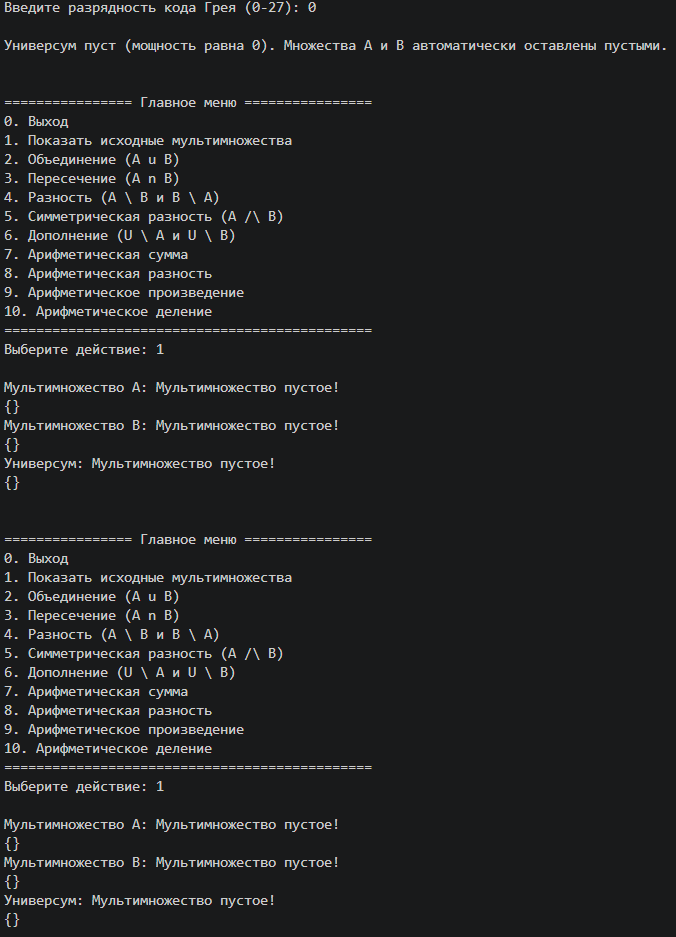
\includegraphics[width=0.85\textwidth]{scenario_empty_universe.png}
		\caption{Работа программы в режиме нулевой разрядности кода Грея ($n = 0$)}
		\label{fig:empty_universe}
	\end{figure}
	
	\subsection{Сценарий 2. Тестирование защиты от некорректного пользовательского ввода}
	
	В рамках сценария проверяется реакция подсистемы валидации \\ \texttt{getValidatedInt()}:
	\begin{enumerate}
		\item Ввод нечисловых символов (\texttt{"abc"}, \texttt{"!?"}) на этапе выбора разрядности;
		\item Ввод отрицательного числа ($-5$ при допустимом минимуме $0$);
		\item Ввод числа, превышающего допустимый диапазон быстродействия ($28$ или $35$ при максимуме $27$);
		\item Попытка задать кратность элемента при ручном заполнении, превышающую оставшуюся емкость данного элемента в сгенерированном универсуме $U$.
	\end{enumerate}
	
	При нарушении формата потока ввода \texttt{cin} программа очищает флаги ошибок вызовом \texttt{cin.clear()}, освобождает входной буфер методом \texttt{cin.ignore()} и выводит сообщение с указанием корректных границ допустимого диапазона, предотвращая зацикливание.
	
	\begin{figure}[H]
		\centering
		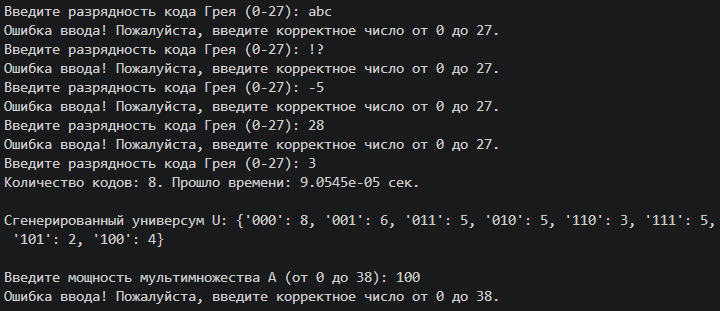
\includegraphics[width=0.85\textwidth]{input_validation.png}
		\caption{Отработка защиты от некорректного пользовательского ввода}
		\label{fig:validation}
	\end{figure}
	На рис.~\ref{fig:validation} показана реакция терминала: ввод символьных строк и чисел вне диапазона $[0, 27]$ блокируется с выводом диагностических предупреждений и повторным запросом ввода до получения корректного значения.
	
	\subsection{Сценарий 3. Генерация универсума и заполнение мультимножеств}
	
	Пользователь задает разрядность $n = 3$. Программа генерирует $N = 2^3 = 8$ комбинаций бинарного кода Грея. Пользователь задает мощности: $|A| = 5$ (ручное заполнение), $|B| = 8$ (автоматическое заполнение).
	При ручном заполнении множества $A$ интерфейс отображает доступную кратность элементов в $U$ и динамически ограничивает максимальный ввод. Множество $B$ наполняется автоматически функцией \texttt{fillAutomatically()} со случайным распределением кратностей с обязательным контролем наличия элементов в универсуме.
	
	На рис.~\ref{fig:filling} показан вывод консоли при генерации 8 кодов Грея, случайном задании кратностей универсума, а также пошаговый процесс ручного ввода множества $A$ с контролем лимитов емкости $U$ и автоматической генерации множества $B$. Полученные мультимножества А и В показаны при вызове пункта 1 меню.
	\begin{figure}[H]
		\centering
		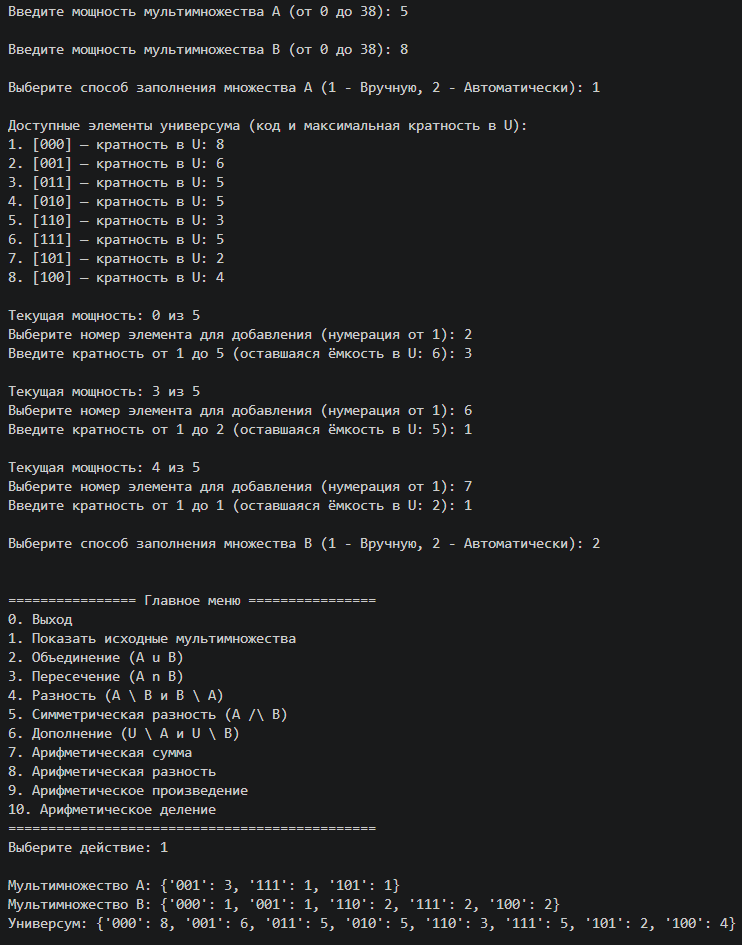
\includegraphics[width=0.85\textwidth]{fill_sets.png}
		\caption{Протокол генерации универсума и наполнения мультимножеств A и B}
		\label{fig:filling}
	\end{figure}
	
	\subsection{Сценарий 4. Проверка теоретико-множественных операций (пункты меню 2--6)}
	На полученных мультимножествах из предыдущих сценариев протестированы операции из пунктов меню 2--6.	Полученные результаты строго согласуются с ручным теоретическим расчетом по формулам, приведенным в подразделе~1.2.
	На рис.~\ref{fig:set_ops1} зафиксированы экранные снимки консоли при вызове пунктов меню 2--4, а на  рис.~\ref{fig:set_ops2} -- пунктов 5 и 6 меню: для каждого пункта отображается правильный результат.
	\begin{figure}[H]
		\centering
		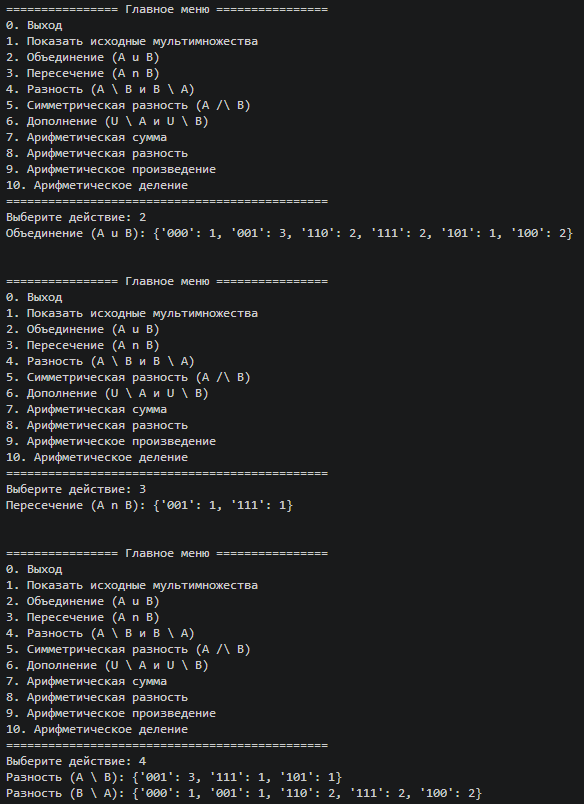
\includegraphics[width=0.85\textwidth]{set_operations1.png}
		\caption{Результаты выполнения теоретико-множественных операций (пункты меню 2--4)}
		\label{fig:set_ops1}
	\end{figure}
	\begin{figure}[H]
		\centering
		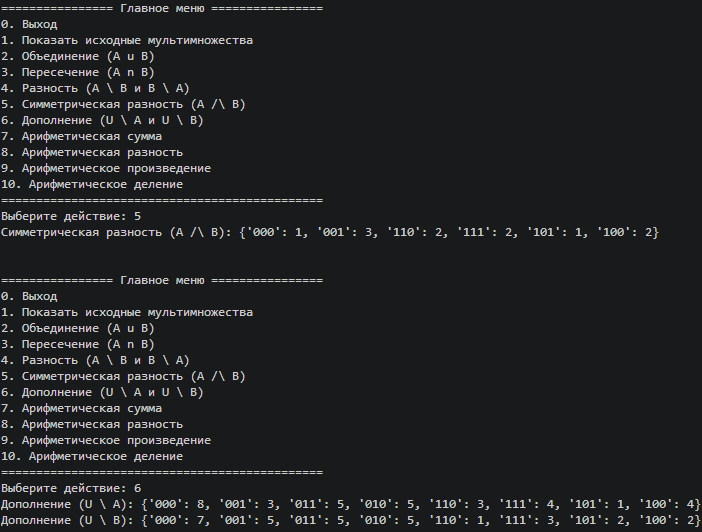
\includegraphics[width=0.85\textwidth]{set_operations2.png}
		\caption{Результаты выполнения теоретико-множественных операций (пункты меню 5 и 6)}
		\label{fig:set_ops2}
	\end{figure}
	
	\subsection{Сценарий 5. Проверка арифметических операций \\ (пункты меню 7--10)}
	
	На полученных мультимножествах из предыдущих сценариев протестированы операции из пунктов меню 7--10. Полученные результаты строго согласуются с ручным теоретическим расчетом по формулам, приведенным в подразделе~1.2.
	На рис.~\ref{fig:arithmetic_ops} зафиксированы экранные снимки консоли при вызове пунктов меню 7--10: для каждого пункта отображается правильный результат.
	
	\begin{figure}[H]
		\centering
		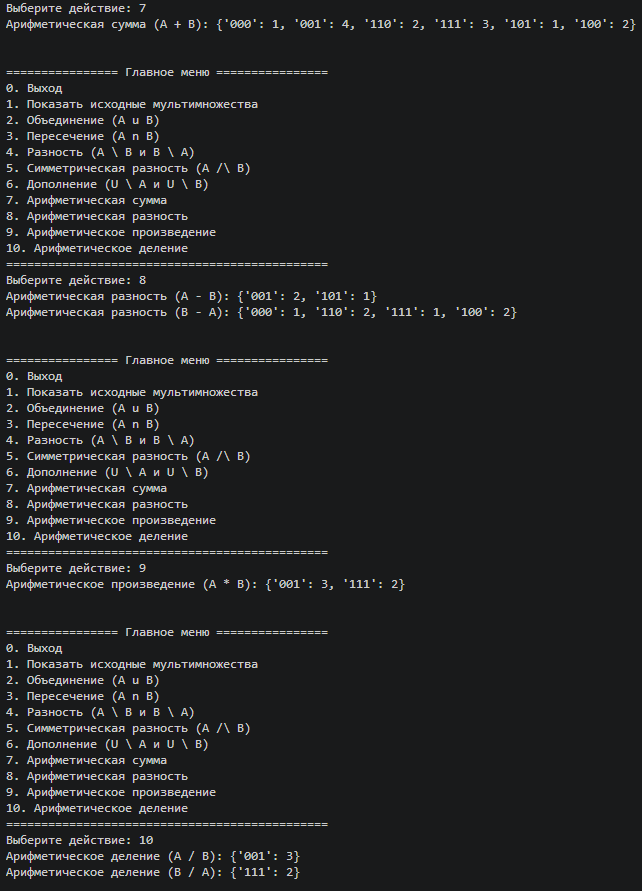
\includegraphics[width=0.85\textwidth]{arithmetic_operations.png}
		\caption{Результаты выполнения арифметических операций (пункты меню 7--10)}
		\label{fig:arithmetic_ops}
	\end{figure}
	
	\subsection{Сценарий 6. Тестирование при большой разрядности и ограничение вывода}
	
	Для проверки масштабируемости программы проведен запуск с повышенной разрядностью. При предельной разрядности $n = 27$ размер носителя составляет $N = 2^{27} = 134\,217\,728$ кодовых комбинаций. Зафиксированное время генерации составило $3.72468$ секунды, что удовлетворяет требованию быстродействия до 5 секунд.
	
	\begin{figure}[H]
		\centering
		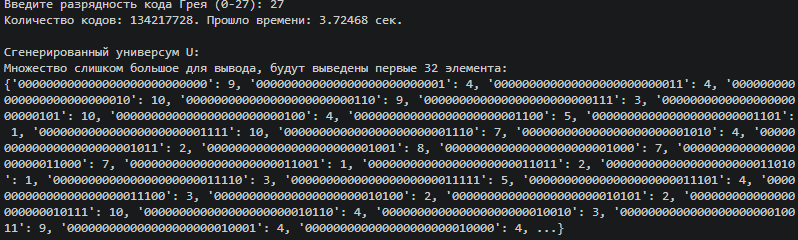
\includegraphics[width=0.85\textwidth]{large_universe_limit.png}
		\caption{Ограничение вывода до 32 элементов и замер времени генерации при больших $n$}
		\label{fig:large_universe}
	\end{figure}
	На рис.~\ref{fig:large_universe} продемонстрирована работа механизма усечения вывода для размерностей более 32 элементов, а также замер времени работы генератора кода Грея при $n = 27$.
	
	\newpage
	\thispagestyle{empty}
	\phantomsection
	\addcontentsline{toc}{section}{Заключение}
	{\LARGE\bf Заключение}\\
	
	В ходе лабораторной работы на языке C++20 разработан программный комплекс для генерации бинарного кода Грея и выполнения полного набора операций над мультимножествами. В рамках реализации спроектирован класс \texttt{MultiSet} на базе вектора кратностей, поддержаны ручной и автоматический режимы ввода, независимая генерация кратностей элементов универсума случайными числами от 1 до 10, а также корректная обработка краевого случая пустого универсума ($n = 0$). По критерию допустимого времени генерации ($\le 5$ с) максимальная разрядность кода Грея зафиксирована равной $n = 27$ со средним временем построения, равном 3.6 секунды. Реализованы все требуемые теоретико-множественные и арифметические операции, обеспечена строгая валидация пользовательского ввода и проведено тестирование, подтвердившее надежность и корректность выполнения программы.
	
	{\bf Достоинства реализованного решения:}
	\begin{itemize}
		\item Высокая скорость доступа к элементам и линейная сложность вычисления операций над мультимножеством.
		\item Лаконичность и безопасность кода благодаря алгоритмам STL (\texttt{std::transform})
	\end{itemize}
	
	{\bf Недостатки решения:}
	\begin{itemize}
		\item Экспоненциальный расход памяти при росте разрядности кода Грея ($N = 2^n$).
		\item Неэффективность плотного вектора для сильно разреженных мультимножеств.
	\end{itemize}
	
	{\bf Масштабирование алгоритма:}
	Для работы с большими универсумами ($n \ge 30$) целесообразно заменить плотный вектор ассоциативным контейнером \texttt{unordered\_map<int, int>}, реализованный на хэш-таблице и не хранящей нулевых элементов. Также для ускорения поэлементной обработки возможно применение параллельных вычислений.
	
	\newpage
	\phantomsection
	\addcontentsline{toc}{section}{Список литературы.}
	
	\begin{thebibliography}{9}
		
		\bibitem{novikov}
		Новиков Ф. А. Дискретная математика для программистов : Учебник для вузов / Ф. А. Новиков. -- 3-е изд. -- СПб. : Питер, 2009. -- 384 с. (Дата обращения -- 10.10.2026)
	
	\end{thebibliography}
	
	\clearpage
	\phantomsection
	\begin{flushleft}
		{\bf Приложение А. Заголовочный файл MultiSet.hpp}
	\end{flushleft}
	\addcontentsline{toc}{section}{Приложение А. Заголовочный файл MultiSet.hpp}
	\label{appendix:A}
	
	\begin{lstlisting}[caption={Заголовочный файл MultiSet.hpp}, label={lst:multiset_hpp}]
		#ifndef SET_HPP
		#define SET_HPP
		
		#include <vector>
		
		class MultiSet
		{
			std::vector<int> counts;
			public:
			MultiSet();
			std::vector<int>::iterator begin()
			{
				return counts.begin();
			}
			int size()
			{
				return counts.size();
			}
			std::vector<int>::iterator end()
			{
				return counts.end();
			}
			int &operator[](size_t pos)
			{
				return counts[pos];
			}
			void resize(size_t new_size, const int val){
				counts.resize(new_size, val);
			}
		};
		
		extern int U_SIZE;
		extern MultiSet multi_universe;
		
		MultiSet uni(MultiSet &A, MultiSet &B);
		MultiSet insertion(MultiSet &A, MultiSet &B);
		MultiSet difference(MultiSet &A, MultiSet &B);
		MultiSet sym_difference(MultiSet &A, MultiSet &B);
		MultiSet complement(MultiSet &A);
		
		MultiSet operator+(MultiSet &A, MultiSet &B);
		MultiSet operator-(MultiSet &A, MultiSet &B);
		MultiSet operator*(MultiSet &A, MultiSet &B);
		MultiSet operator/(MultiSet &A, MultiSet &B);
		
		#endif
	\end{lstlisting}
	
	\clearpage
	\phantomsection
	\begin{flushleft}
		{\bf Приложение Б. Файл реализации MultiSet.cpp}
	\end{flushleft}
	\addcontentsline{toc}{section}{Приложение Б. Файл реализации MultiSet.cpp}
	\label{appendix:B}
	
	\begin{lstlisting}[caption={Файл реализации MultiSet.cpp}, label={lst:multiset_cpp}]
	#include "MultiSet.hpp"
	#include <algorithm>
	#include <cmath>
	#include <iostream>
	
	using namespace std;
	
	MultiSet::MultiSet() : counts(U_SIZE, 0) {}
	
	// объединение: max(a, b)
	MultiSet uni(MultiSet &A, MultiSet &B)
	{
		MultiSet result;
		transform(A.begin(), A.end(), B.begin(), result.begin(), [](int a, int b)
		{ return max(a, b); });
		return result;
	}
	
	// пересечение: min(a, b)
	MultiSet insertion(MultiSet &A, MultiSet &B)
	{
		MultiSet result;
		transform(A.begin(), A.end(), B.begin(), result.begin(), [](int a, int b)
		{ return min(a, b); });
		return result;
	}
	
	// дополнение: m - a, m - кратность эл-та в универсуме
	MultiSet complement(MultiSet &A)
	{
		MultiSet result;
		transform(A.begin(), A.end(), multi_universe.begin(), result.begin(), [](int a, int m)
		{ return m - a; });
		return result;
	}
	
	// разность: A n -B
	MultiSet difference(MultiSet &A, MultiSet &B)
	{
		MultiSet notB = complement(B);
		return insertion(A, notB);
	}
	
	// симметрическая разность: (A u B) \ (A n B)
	MultiSet sym_difference(MultiSet &A, MultiSet &B)
	{
		MultiSet AuB = uni(A, B);
		MultiSet AnB = insertion(A, B);
		return difference(AuB, AnB);
	}
	
	// арифметическая сумма
	MultiSet operator+(MultiSet &A, MultiSet &B)
	{
		MultiSet result;
		transform(A.begin(), A.end(), B.begin(), result.begin(), [](int a, int b)
		{ return a + b; });
		
		transform(result.begin(), result.end(), multi_universe.begin(), result.begin(), [](int sum, int m)
		{ return min(sum, m); });
		return result;
	}
	
	// арифметическая разность
	MultiSet operator-(MultiSet &A, MultiSet &B)
	{
		MultiSet result;
		transform(A.begin(), A.end(), B.begin(), result.begin(), [](int a, int b)
		{ return max(0, a - b); });
		return result;
	}
	
	// арифметическое произведение
	MultiSet operator*(MultiSet &A, MultiSet &B)
	{
		MultiSet result;
		for (int i = 0; i < U_SIZE; i++)
		{
			result[i] = min(A[i] * B[i], multi_universe[i]);
		}
		return result;
	}
	
	// арифметическое деление
	MultiSet operator/(MultiSet &A, MultiSet &B)
	{
		MultiSet result;
		transform(A.begin(), A.end(), B.begin(), result.begin(), [](int a, int b)
		{ return (b == 0) ? 0 : (a / b); });
		return result;
	}
	\end{lstlisting}
	
	\clearpage
	\phantomsection
	\begin{flushleft}
		{\bf Приложение В. Файл точки входа и интерфейса main.cpp}
	\end{flushleft}
	\addcontentsline{toc}{section}{Приложение В. Файл точки входа и интерфейса main.cpp}
	\label{appendix:C}
	
	\begin{lstlisting}[caption={Файл точки входа и интерфейса main.cpp}, label={lst:main_cpp}]
	#include <string>
	#include <limits>
	#include <iostream>
	#include <vector>
	#include <bitset>
	#include <format>
	#include <algorithm>
	#include <chrono>
	#include "MultiSet.hpp"
	
	int U_SIZE = 0;
	MultiSet multi_universe;
	
	using namespace std;
	int getValidatedInt(const string &prompt = "", int min_val = 0, int max_val = numeric_limits<int>::max())
	{
		int value;
		while (true)
		{
			cout << prompt;
			if (cin >> value && value >= min_val && value <= max_val)
			{
				cin.ignore(numeric_limits<streamsize>::max(), '\n');
				return value;
			}
			cout << "Ошибка ввода! Пожалуйста, введите корректное число от " << min_val << " до " << max_val << ".\n";
			cin.clear();
			cin.ignore(numeric_limits<streamsize>::max(), '\n');
		}
	}
	
	int Q(int i)
	{
		int q = 1;
		int j = i;
		while (j % 2 == 0)
		{
			j = j / 2;
			q = q + 1;
		}
		return q;
	}
	
	void generateGrayCode(int n, vector<int> &target)
	{
		target.clear();
		int B = 0;
		target.push_back(B);
		
		int total_steps = 1 << n;
		
		for (int i = 1; i < total_steps; i++)
		{
			// n=8
			// p_index = 1
			// B[1]
			// B=00000000
			// B=01000000
			int p_index = Q(i) - 1;
			B ^= 1 << p_index;
			target.push_back(B);
		}
	}
	
	void printBinary(int code, int bitrate)
	{
		for (int i = bitrate - 1; i >= 0; i--)
		{
			cout << ((code >> i) & 1);
		}
	}
	
	void printMultiSet(MultiSet &ms, const vector<int> &u, int bitrate)
	{
		if (ms.size() == 0)
		{
			cout << "Мультимножество пустое!\n";
		}
		
		size_t limit = u.size();
		bool is_truncated = false;
		
		if (u.size() > 32)
		{
			cout << "\nМножество слишком большое для вывода, будут выведены первые 32 элемента:\n";
			limit = 32;
			is_truncated = true;
		}
		
		bool first = true;
		cout << "{";
			for (size_t i = 0; i < limit; ++i)
			{
				if (ms[i] > 0)
				{
					if (!first)
					cout << ", ";
					cout << "'";
					printBinary(u[i], bitrate);
					cout << "': " << ms[i];
					first = false;
				}
			}
			
			if (is_truncated)
			{
				if (!first)
				cout << ", ...";
				else
				cout << "...";
			}
			cout << "}\n";
	}
	
	long long createUniverse(MultiSet &u)
	{
		srand(time(nullptr));
		u.resize(U_SIZE, 0);
		if (U_SIZE == 0)
		return 0;
		long long total_capacity = 0;
		for (int i = 0; i < U_SIZE; ++i)
		{
			u[i] = 1 + rand() % 10; // случайное число от 1 до 10
			total_capacity += u[i];
		}
		return total_capacity;
	}
	
	void fillManually(MultiSet &ms, const vector<int> &universe, int bitrate, int target_capacity)
	{
		int current_capacity = 0;
		
		cout << "\nДоступные элементы универсума (код и максимальная кратность в U):\n";
		for (int i = 0; i < universe.size(); ++i)
		{
			cout << i + 1 << ". [";
			printBinary(universe[i], bitrate);
			cout << "] — кратность в U: " << multi_universe[i] << "\n";
		}
		
		while (current_capacity < target_capacity)
		{
			cout << "\nТекущая мощность: " << current_capacity << " из " << target_capacity << "\n";
			int idx = getValidatedInt("Выберите номер элемента для добавления (нумерация от 1): ", 1, universe.size()) - 1;
			
			int remaining_in_u = multi_universe[idx] - ms[idx];
			if (remaining_in_u <= 0)
			{
				cout << "Этот элемент недоступен (оставшаяся ёмкость в универсуме равна 0). Выберите другой элемент.\n";
				continue;
			}
			
			int max_allowed = min(remaining_in_u, target_capacity - current_capacity);
			string prompt = format("Введите кратность от 1 до {} (оставшаяся ёмкость в U: {}): ", max_allowed, remaining_in_u);
			int count = getValidatedInt(prompt, 1, max_allowed);
			
			ms[idx] += count;
			current_capacity += count;
		}
	}
	
	void fillAutomatically(MultiSet &ms, const vector<int> &universe, int target_capacity)
	{
		int current_capacity = 0;
		while (current_capacity < target_capacity)
		{
			int idx = rand() % U_SIZE;
			if (ms[idx] < multi_universe[idx])
			{
				ms[idx]++;
				current_capacity++;
			}
		}
	}
	
	int main(int argc, char const *argv[])
	{
		// при bitrate = 28 время вычисления кода грея составило в среднем 7.3 секунды. при 27 - 3.6 сек.
		int bitrate = getValidatedInt("Введите разрядность кода Грея (0-27): ", 0, 27);
		auto start = chrono::steady_clock::now();
		MultiSet A, B;
		vector<int> universe;
		if (bitrate == 0)
		{
			cout << "\nУниверсум пуст (мощность равна 0). Множества A и B автоматически оставлены пустыми.\n";
		}
		else
		{
			universe.resize(1 << bitrate, 0);
			generateGrayCode(bitrate, universe);
			U_SIZE = universe.size();
			
			A.resize(U_SIZE, 0);
			B.resize(U_SIZE, 0);
			
			long long total_u_capacity = createUniverse(multi_universe);
			
			auto end = chrono::steady_clock::now();
			chrono::duration<double> elapsed = end - start;
			cout << "Количество кодов: " << U_SIZE << ". Прошло времени: " << elapsed.count() << " сек.\n";
			
			cout << "\nСгенерированный универсум U: ";
			printMultiSet(multi_universe, universe, bitrate);
			
			int lower_capacity = 0;
			int upper_capacity;
			if (100LL < total_u_capacity)
			upper_capacity = 100;
			else
			upper_capacity = total_u_capacity;
			
			int capacityA = getValidatedInt(format("\nВведите мощность мультимножества A (от {} до {}): ", lower_capacity, upper_capacity),
			lower_capacity, upper_capacity);
			int capacityB = getValidatedInt(format("\nВведите мощность мультимножества B (от {} до {}): ", lower_capacity, upper_capacity),
			lower_capacity, upper_capacity);
			
			if (capacityA > 0)
			{
				int choiceA = getValidatedInt("\nВыберите способ заполнения множества A (1 - Вручную, 2 - Автоматически): ", 1, 2);
				if (choiceA == 1)
				fillManually(A, universe, bitrate, capacityA);
				else
				fillAutomatically(A, universe, capacityA);
			}
			if (capacityB > 0)
			{
				int choiceB = getValidatedInt("\nВыберите способ заполнения множества B (1 - Вручную, 2 - Автоматически): ", 1, 2);
				if (choiceB == 1)
				fillManually(B, universe, bitrate, capacityB);
				else
				fillAutomatically(B, universe, capacityB);
			}
		}
		
		while (true)
		{
			cout << "\n\n================ Главное меню ================\n";
			cout << "0. Выход\n";
			cout << "1. Показать исходные мультимножества\n";
			cout << "2. Объединение (A u B)\n";
			cout << "3. Пересечение (A n B)\n";
			cout << "4. Разность (A \\ B и B \\ A)\n";
			cout << "5. Симметрическая разность (A /\\ B)\n";
			cout << "6. Дополнение (U \\ A и U \\ B)\n";
			cout << "7. Арифметическая сумма\n";
			cout << "8. Арифметическая разность\n";
			cout << "9. Арифметическое произведение\n";
			cout << "10. Арифметическое деление\n";
			cout << "==============================================\n";
			
			int menuChoice = getValidatedInt("Выберите действие: ", 0, 10);
			
			if (menuChoice == 0)
			{
				cout << "Программа завершена.\n";
				break;
			}
			
			MultiSet result;
			
			switch (menuChoice)
			{
				case 1:
				cout << "\nМультимножество A: ";
				printMultiSet(A, universe, bitrate);
				cout << "Мультимножество B: ";
				printMultiSet(B, universe, bitrate);
				cout << "Универсум: ";
				printMultiSet(multi_universe, universe, bitrate);
				break;
				case 2:
				result = uni(A, B);
				cout << "Объединение (A u B): ";
				printMultiSet(result, universe, bitrate);
				break;
				case 3:
				result = insertion(A, B);
				cout << "Пересечение (A n B): ";
				printMultiSet(result, universe, bitrate);
				break;
				case 4:
				result = difference(A, B);
				cout << "Разность (A \\ B): ";
				printMultiSet(result, universe, bitrate);
				
				result = difference(B, A);
				cout << "Разность (B \\ A): ";
				printMultiSet(result, universe, bitrate);
				break;
				case 5:
				result = sym_difference(A, B);
				cout << "Симметрическая разность (A /\\ B): ";
				printMultiSet(result, universe, bitrate);
				break;
				case 6:
				result = complement(A);
				cout << "Дополнение (U \\ A): ";
				printMultiSet(result, universe, bitrate);
				
				result = complement(B);
				cout << "Дополнение (U \\ B): ";
				printMultiSet(result, universe, bitrate);
				break;
				case 7:
				result = A + B;
				cout << "Арифметическая сумма (A + B): ";
				printMultiSet(result, universe, bitrate);
				break;
				case 8:
				result = A - B;
				cout << "Арифметическая разность (A - B): ";
				printMultiSet(result, universe, bitrate);
				
				result = B - A;
				cout << "Арифметическая разность (B - A): ";
				printMultiSet(result, universe, bitrate);
				break;
				case 9:
				result = A * B;
				cout << "Арифметическое произведение (A * B): ";
				printMultiSet(result, universe, bitrate);
				break;
				case 10:
				result = A / B;
				cout << "Арифметическое деление (A / B): ";
				printMultiSet(result, universe, bitrate);
				
				result = B / A;
				cout << "Арифметическое деление (B / A): ";
				printMultiSet(result, universe, bitrate);
				break;
			}
		}
		
		return 0;
	}
	
	\end{lstlisting}
	
	\clearpage
	\phantomsection
	\begin{flushleft}
		{\bf Приложение Г. Скрипт сборки CMakeLists.txt}
	\end{flushleft}
	\addcontentsline{toc}{section}{Приложение Г. Скрипт сборки CMakeLists.txt}
	\label{appendix:D}
	
	\begin{lstlisting}[caption={Скрипт сборки CMakeLists.txt}, label={lst:cmakelists}]
		cmake_minimum_required(VERSION 3.20.0)
		set (CMAKE_CXX_STANDARD 20)
		project(lab1 LANGUAGES CXX)
		
		set(CMAKE_CXX_FLAGS "-fsanitize=address -fno-omit-frame-pointer -O1")
		
		add_library(mylib STATIC 
		src/MultiSet.hpp
		src/MultiSet.cpp
		)
		
		add_executable(main 
		src/main.cpp
		)
		
		target_link_libraries(main mylib)
		
		file(GENERATE 
		OUTPUT "${CMAKE_CURRENT_BINARY_DIR}/run_test.sh"
		CONTENT "cat ../test_data.txt | ./main\n"
		)
	\end{lstlisting}
	
\end{document}